%&latex
%
\documentclass[../template.tex]{subfiles}
%\usepackage{graphicx}

\begin{document}

\chapter{Integrals of complex variables}
In this chapter we discuss several techniques for computing integrals on the complex plane.

\section{Fourier Transform}
\label{sec:fourier}
One of the most frequent kind of complex integral is given by the \textit{Fourier Transform} (FT). Let $f(x) \in L_2(\mathbb{R})$ be a square-integrable function. Then the Fourier transform maps $f(x)$ to another function $\tilde{f}(k)$ defined as follows: \marginpar{Fourier transform}
\begin{align} \label{eqn:fourier-def}
    \mathcal{F}[f(x)](k) = \tilde{f}(k) \equiv \int_{\mathbb{R}} e^{-ikx} f(x) \dd{x} \qquad f \in L_2(\mathbb{R})
\end{align}
Similarly, it is possible to define the \textit{inverse Fourier transform}, linking $\tilde{f}(k)$ back to $f(x)$: \marginpar{Inverse Fourier transform}
\begin{align*}
    \mathcal{F}^{-1}[\tilde{f}(k)](x) = f(x) = \frac{1}{2\pi} \int_{\mathbb{R}} e^{ikx} \tilde{f}(k) \dd{k} 
\end{align*} 
The $2 \pi$ factor is needed for normalization, so that:
\begin{align}
    \mathcal{F}^{-1}[\mathcal{F}[f(x)](k)](x) = f(x) \label{eqn:inverse-property}
\end{align}
As long as (\ref{eqn:inverse-property}) is satisfied, any different \marginpar{Conventions} definition of the Fourier transforms is acceptable. For example, it is possible to \textit{switch} the signs in the $e^{ikx}$, or split differently the normalization factor between $\mathcal{F}$ and $\mathcal{F}^{-1}$. 

\subsection{Refresher on functional analysis}
The definition (\ref{eqn:fourier-def}) is quite limited, as several interesting functions are not in $L_2(\mathbb{R})$ - for example $\sin(x)$, $\cos(x)$, $\theta(x)$. Fortunately, it is possible to extend the Fourier transform by considering \textit{generalized functions} (\textbf{distributions}).   

\medskip


We start by defining a space $\mathcal{S}(\mathbb{R})$ (Schwartz space)\marginpar{Schwartz space} containing all functions $\varphi \in C^{\infty}(\mathbb{R})$ that are \textit{rapidly decreasing}, i.e. such that $\sup_{x \in \mathbb{R}} |x^\alpha \varphi^{(\beta)}(x)| < \infty$ $\forall \alpha, \beta \in \mathbb{N}$. These are also called \textit{test functions}. 

\medskip

Then a \textbf{tempered distribution}\marginpar{Tempered distributions} $T$ is a \textbf{continuous} \textbf{linear} mapping $\mathcal{S}(\mathbb{R}) \to \mathbb{R}$. So it is possible to \q{apply} a distribution $T$ to any test function $\varphi \in \mathcal{S}(\mathbb{R})$, resulting in a real number, denoted with $\langle T, \varphi \rangle$.

\medskip

The choice of $\mathcal{S}$ is made expressly so that the Fourier transform is a linear and invertible operator on $\mathcal{S}$. However, other choices can be made for the space of test functions. For example, one can take the set $\mathcal{D}$ of all functions with \textit{compact support}, i.e. that vanish (along with all their derivatives) outside a compact region. 

\medskip

We can now see that distributions \textit{generalize} the concept of function. We start by noting that any \textbf{locally integrable} function $f \colon \mathbb{R} \to \mathbb{R}$ can be used to define a distribution, by considering its inner product with a test function:  
\begin{align}
    \langle T_f, \varphi \rangle \equiv \int_{\mathbb{R}} \dd{x} f(x)\varphi(x) \qquad \forall \varphi \in \mathcal{S}(\mathbb{R}) \label{eqn:regular-dist}
\end{align}
Distributions that can be defined like this are called \textbf{regular}. 

\begin{expl}In the \textbf{complex} case, where $f \colon \mathbb{R} \to \mathbb{C}$, we instead use the Hermitian inner product:
    \begin{align*}
        \langle T_f, \varphi \rangle = \int_{\mathbb{R}} \dd{x} f(x)^* \varphi(x)
    \end{align*} 
    where $f(x)^*$ is the complex conjugate of $f(x)$. The choice of the \textit{position} of this conjugate (on the first or second entry) is a convention. Physicists tend to use the first position (due to Dirac notation), while mathematicians the second one.
\end{expl}

Not all distributions are regular: in general, it is not possible to find a function $f(x)$ for a generic distribution $T$ such that (\ref{eqn:regular-dist}) is satisfied. The distributions for which this is not possible are called \textbf{singular}.

\medskip

The simplest (and most important) singular distribution is the \textbf{Dirac Delta} \marginpar{\vspace{3em}Dirac Delta}\index{Dirac Delta} $\delta(x)$, defined as follows:
\begin{align*}
    \langle \delta, \varphi \rangle \equiv \varphi(0) \qquad \varphi \in S(\mathbb{R})
\end{align*} 
In other words, applying the $\delta$ to any test function $\varphi$ returns the value of $\varphi$ at $0$.

In practice, we often write \textit{formally}:
\begin{align*}
    \langle \delta, \varphi \rangle = \int_{\mathbb{R}} \delta(x) \varphi(x) \dd{x}
\end{align*}
\textit{as if} $\delta(x)$ were a function (but keep in mind that it isn't). This expression is often just a \textit{shortcut} for quickly reaching useful results, as we will see in the following.

\medskip

The point of defining \textit{distributions} is that they provide a way to extend rigorously may operations that cannot be done on normal functions.  One such example is differentiation. Given a distribution $T$, its \textbf{distributional derivative} is defined as:\marginpar{\vspace{1em}Distributional derivative}
\begin{align} \label{eqn:dist-derivative}
    \langle T', \varphi \rangle \equiv - \langle T, \varphi' \rangle \qquad \forall \varphi \in S(\mathbb{R})
\end{align}  
This is done so that, for a \textit{regular} distribution $T_f$, that result comes from integration by parts:
\begin{align} \label{eqn:construction}
    \langle T'_f, \varphi \rangle = \int_{\mathbb{R}} f'(x) \varphi(x) \dd{x} = \cancel{f(x) \varphi(x) \Big|_{-\infty}^{+\infty}} - \int_{\mathbb{R}} f(x) \varphi'(x) = - \langle T_f, \varphi' \rangle
\end{align} 
For a singular distribution we use directly the definition (\ref{eqn:dist-derivative}), as the construction in (\ref{eqn:construction}) has no meaning (but still, sometimes we will write it nonetheless, as a merely \textit{formal} expression).

\medskip

In the distributional sense, it is possible to differentiate the \textbf{Heaviside function}\index{Heaviside function}\marginpar{\vspace{4.5em}Heaviside step function} $\theta(x)$:
\begin{align} \label{eqn:heaviside-def}
    \theta(x) \equiv \begin{cases}
        1 & x > 0\\
        \frac{1}{2} & x=0\\
        0 & x < 0 
    \end{cases}
\end{align}
As $\theta(x)$ is locally integrable, we can define a corresponding distribution - that we denote with the same symbol $\theta$. Then:
\begin{align}\nonumber
    \langle \theta', \varphi \rangle &= - \langle \theta, \varphi' \rangle = -\int_{\mathbb{R}} \theta(x) \varphi'(x) \dd{x} = -\int_0^{+\infty} \varphi'(x) \dd{x} = -[\cancel{\varphi(+\infty)}-\varphi(0)] =\\
    &= \varphi(0) = \langle \delta | \varphi \rangle \label{eqn:theta-deriv}
\end{align}
So $\theta' = \delta$ \textit{in the distributional sense} - i.e. applying $\theta'$ or $\delta$ to any test function $\varphi$ leads to the same result.

\subsection{Fourier transform of distributions}

We are finally ready to extend the \textbf{Fourier Transform} to tempered distributions.\marginpar{\vspace{3em}Fourier Transform of distributions} In fact, $S(\mathbb{R})$ has been chosen\footnote{More precisely, the Fourier transform is an \textit{automorphism} of $\mathcal{S}$, i.e. it is linear and invertible} such that any $\varphi(x) \in S(\mathbb{R})$ has a well-defined transform $\tilde{\varphi}(k)$. Then we define the Fourier transform of a distribution as follows:
\begin{align*}
    \langle \mathcal{F}[T], \varphi \rangle \equiv 2\pi\langle T, \mathcal{F}^{-1}[\varphi] \rangle
\end{align*}

Again, this comes from the expression for regular distributions:
\begin{align*}
    \langle \mathcal{F}[T_f], \varphi \rangle &= \int_{\mathbb{R}} \dd{k} \{\mathcal{F}[f(x)](k)\}^* \varphi(k) = \int_{\mathbb{R}} \dd{k} \int_{\mathbb{R}} \dd{x} \left[e^{-ikx} f(x)\right]^* \varphi(x) =\\
    &= \int_{\mathbb{R}} \dd{x} f(x) \int_{\mathbb{R}} \dd{k} e^{ikx}  \varphi(k) = \int_{\mathbb{R}} 2\pi f(x) \mathcal{F}^{-1}[\varphi(k)](x) = 2 \pi\langle T, \mathcal{F}^{-1}[\varphi]  \rangle
\end{align*}

Note that:
\begin{align}\label{eqn:unitary}
    \langle \mathcal{F}[T], \mathcal{F}[\varphi] \rangle = 2\pi \langle T, \mathcal{F}^{-1} \mathcal{F}[\varphi] \rangle = 2 \pi \langle T, \varphi \rangle
\end{align}

\subsubsection{Delta transform}
Finally, we can use all this machinery to compute Fourier transforms of some \textit{generalized functions}. We start with the $\delta$:
\begin{align*}
    \langle \mathcal{F}[\delta], \varphi \rangle = 2 \pi\langle \delta, \mathcal{F}^{-1}[\varphi]\rangle = 2\pi\mathcal{F}^{-1}[\varphi(x)](0)
\end{align*}
where:
\begin{align*}
    \mathcal{F}^{-1}[\varphi(x)](k) = \frac{1}{2\pi} \int_{\mathbb{R}} \dd{x} e^{ikx} \varphi(x) \Rightarrow 2 \pi\mathcal{F}^{-1}[\varphi(x)](0) = \int_{\mathbb{R}} \dd{x} \varphi(x) = \langle 1, \varphi \rangle 
\end{align*}
And so $\mathcal{F}[\delta] = 1$. 

\medskip

Note that the same result could be obtained in a simpler way by treating $\delta$ as a \q{formal function}:
\begin{align*}
    \mathcal{F}[\delta](k) = \int_{\mathbb{R}} e^{-ikx} \delta(x) = e^{-ik 0} =  1
\end{align*}
This leads to an equivalent definition for the $\delta$ \q{function}:
\begin{align*}
    \delta(x) = \mathcal{F}^{-1}[1](x) = \frac{1}{2\pi} \int_{\mathbb{R}} e^{ikx} \dd{k}
\end{align*}
Also, note that:
\begin{align} \label{eqn:1-transform}
    \mathcal{F}[1](k) = \int_{\mathbb{R}} e^{-ikx} \dd{x} = \int_{\mathbb{R}} e^{ikx} \dd{x} = \textcolor{Red}{2 \pi} \left( \frac{1}{\textcolor{Red}{2 \pi}} \int_{\mathbb{R}} e^{ikx}  \right) = 2\pi \delta(k)
\end{align}

\subsubsection{Heaviside transform}
We can use the result for the $\delta$ to aid the computation of $\mathcal{F}[\theta]$, where $\theta(x)$ is the regular distribution defined from (\ref{eqn:heaviside-def}). We have already seen in (\ref{eqn:theta-deriv}) that $\theta' = \delta$. So, we can use the formula for the Fourier transform of a derivative\marginpar{\vspace{2em}Fourier transform of a derivative} (which naturally generalizes to distributions):
\begin{align} \label{eqn:derivative-property}
    \mathcal{F}[T'] = ik \tilde{T}
\end{align}
In our case:
\begin{align} \label{eqn:theta-transf1}
    \mathcal{F}[\theta'] \underset{(\ref{eqn:theta-deriv})}{=}  \mathcal{F}[\delta] = 1 = ik \tilde{\theta}
\end{align}


However, (\ref{eqn:theta-transf1}) cannot be used to reconstruct $\tilde{\theta}$ by itself, that is we cannot just \q{solve by $\tilde{\theta}$} and write:
\begin{align} \label{eqn:wrong-theta-transform}
    \tilde{\theta}(k) = \frac{1}{ik} 
\end{align}

In fact, consider a different $\theta^*(x) \equiv \theta(x) + c$, with $c \in \mathbb{R}$ constant. Their derivatives coincide, and so formula (\ref{eqn:theta-transf1}) would give the same result for both of them. However:
\begin{align*}
    \mathcal{F}[\theta^*(x)](k) = \mathcal{F}[\theta(x)](k) + \mathcal{F}[c](k) = \tilde{\theta}(k) + c \delta(k) \neq \tilde{\theta}(k)
\end{align*}
So we are missing a $\delta$ term, meaning that the correct Fourier transform should be:\marginpar{\vspace{2em}Inversion formula}
\begin{align}\label{eqn:full-theta-tilda}
    \tilde{\theta}(k) = \mathcal{P}\left(\frac{1}{ik} \right) + c \delta(k)
\end{align}
for some constant $c$. $\mathcal{P}$ denotes the Cauchy principal value, which needs to be used to \q{fix} the singularity at $k=0$ (see the following green boxes for the details).

\medskip

There are several ways to fix $c$ in (\ref{eqn:full-theta-tilda}). One of the quickest is to reason \textit{with symmetries}.

Let $f$ be an even function\marginpar{1. Fix $c$ (symmetries)} (i.e. a gaussian). Symmetry is preserved by the Fourier transform, and so:
\begin{align}
    \langle \tilde{\theta}, \tilde{f} \rangle = \mathcal{P} \int_{\mathbb{R}} \frac{1}{ik} \tilde{f}(k) \dd{k} + c \langle \delta, \tilde{f} \rangle = c \tilde{f}(0) = c \int_{\mathbb{R}} f(x) \dd{x} \label{eqn:scalar1}
\end{align}
The principal value vanishes because $\tilde{f}$ is even (as $f$ is even). The corresponding scalar product without the Fourier transforms is:\begin{align}
    \langle \theta, f \rangle = \int_{0}^{+\infty} f(x) \dd{x} \underset{(a)}{=}  \frac{1}{2} \int_{\mathbb{R}} f(x) \dd{x} \label{eqn:scalar2} 
\end{align}
where in (a) we again used the symmetry of $f$. Then, recalling (\ref{eqn:unitary}), we have:
\begin{align*}
    \langle \tilde{\theta}, \tilde{f} \rangle = 2\pi \langle \theta, f \rangle \Rightarrow c\int_{\mathbb{R}} f(x) \dd{x} = \frac{2 \pi}{2} \int_{\mathbb{R}} f(x) \dd{x} \Rightarrow c = \pi 
\end{align*}
(Note that $c$ depends on the choice we made for the normalization in the Fourier transforms).

\medskip

A similar argument\marginpar{2. Fix $c$ with symmetries and $\operatorname{sgn}(x)$} can be made noting that $\theta(x)$ is just a scaled and shifted $\operatorname{sgn}$ function, which is odd:
\begin{align*}
    \theta(x) = \frac{1}{2} +  \frac{1}{2}\operatorname{sgn}(x) \qquad
    \operatorname{sgn}(x) = \begin{cases}
        1 & x > 0\\
        0 & x = 0\\
        -1 & x < 0
    \end{cases} 
\end{align*} 
By linearity we have:
\begin{align}
    \tilde{\theta}(k) = \mathcal{F}\left(\frac{1}{2}\right) + \frac{1}{2} \mathcal{F}[\operatorname{sgn}(x)](k) \label{eqn:theta-transform2}
\end{align}
Noting that $\operatorname{sgn}' = 2 \delta$ and using (\ref{eqn:derivative-property}) leads to:
\begin{align*}
    2 = ik \mathcal{F}[\operatorname{sgn}](k)
\end{align*}
Inverting with (\ref{eqn:full-theta-tilda}), we have:
\begin{align*}
    \mathcal{F}[\operatorname{sgn}](k) = \mathcal{P}\left(\frac{2}{ik} \right) + c \delta(k) =\mathcal{P}\left(\frac{2}{ik} \right) \ 
\end{align*}
As this time $c$ must be $0$, otherwise $\mathcal{F}[\operatorname{sgn}](k)$ wouldn't be odd (the $\delta$ is \textit{even}). Substituting in (\ref{eqn:theta-transform2}) we have:
\begin{align*}
    \tilde{\theta}(k) = \frac{1}{2} \underbrace{\mathcal{F}[1] }_{2 \pi}+\frac{1}{\cancel{2}} \mathcal{P}\left(\frac{\cancel{2}}{ik} \right) = \mathcal{P}\left(\frac{1}{ik} \right)  + \pi \delta(k)
\end{align*}

\begin{expl}\textbf{Why is (\ref{eqn:wrong-theta-transform}) wrong?} There are two main reasons:
\begin{itemize}
    \item $1/(ik)$ is not locally integrable (as it diverges for $k=0$), so it cannot be used to define a distribution, such as $\tilde{\theta}$. This can be solved by using the \textit{principal part} of $1/(ik)$ instead. 
    \item The most general solution to the equation $xT = 1$, where $T$ is a tempered distribution, is not just $T = \mathcal{P} (1/x)$, but:
    \begin{align*}
        T = \mathcal{P}\left(\frac{1}{x} \right) + c \delta
    \end{align*}
    for some constant $c \in \mathbb{R}$.
\end{itemize}

First, to be precise, the product of a function, such as $f(x) = x$, with a distribution $T$ is \textit{defined} as the following distribution:
\begin{align} \label{eqn:dist-mult}
    \langle f(x)T, \varphi \rangle \equiv \langle T, f(x) \varphi \rangle
\end{align} 
where $f(x)$ must be such that $f(x) \varphi \in \mathcal{S}$ $\forall \varphi \in \mathcal{S}$, which is indeed the case for any polynomial. 

Now consider the \textit{distributional} equation $x T =1$. If we apply \textit{both sides} to some test function $\varphi$, we have:
\begin{align} \label{eqn:division}
    \langle T, x \varphi \rangle = \langle 1, \varphi \rangle = \int_{\mathbb{R}} \varphi(x) \dd{x}
\end{align}  
The problem of \textit{finding} $T$ satisfying (\ref{eqn:division}) is called the (distributional) \textbf{division problem}. To solve it, we want to reduce the equation to something in the form of $x T' = 0$, that can then be solved. So we rewrite the rhs as follows:
\begin{align*}
    \int_{\mathbb{R}} \varphi(x) \dd{x} = \lim_{\epsilon \to 0^+} \int_{\mathbb{R} \setminus [-\epsilon, \epsilon]} \varphi(x) \dd{x} = \lim_{\epsilon \to 0^+} \int_{\mathbb{R}\setminus [-\epsilon, \epsilon]} \frac{x \varphi(x)}{x} \dd{x}
\end{align*}
Then we define the \textbf{principal value distribution} $\mathcal{P}(1/x)$ as:
\begin{align*}
    \langle \mathcal{P}\left(\frac{1}{x} \right), \varphi\rangle = \lim_{\epsilon \to 0^+} \int_{\mathbb{R} \setminus [-\epsilon, \epsilon]} \frac{\varphi(x)}{x} \dd{x} 
\end{align*} 
so that:
\begin{align*}
    \int_{\mathbb{R}}\varphi(x) \dd{x} = \langle \mathcal{P}\left(\frac{1}{x}\right), x\varphi \rangle
\end{align*}
Substituting back in (\ref{eqn:division}) and rearranging we get:
\begin{align*}
    \langle T, x \varphi \rangle = \langle \mathcal{P}\left(\frac{1}{x}\right), x\varphi \rangle \Rightarrow \langle T - \mathcal{P}\left(\frac{1}{x} \right), x \varphi \rangle = 0 \underset{(\ref{eqn:dist-mult})}{\Rightarrow}  
    x\left[T - \mathcal{P}\left(\frac{1}{x} \right)\right] = 0
\end{align*}
%Show solution xT = 0. From https://see.stanford.edu/materials/lsoftaee261/book-fall-07.pdf in 4.13.1 sec. and https://math.stackexchange.com/questions/678457/distribution-solution-to-xt-0-in-schwartz-space
%Extend to xT = 1 with https://math.stackexchange.com/questions/2962209/solve-the-distribution-equation-xt-1 (introducing Cauchy principal part)
     
%Also look up "division problem" for distributions

    All that's left is to solve:
    \begin{align}
        x T' = 0 \label{eqn:reduced-div}
    \end{align}
    with $T' = T - \mathcal{P}(1/x)$. We will now see that the general solution of (\ref{eqn:reduced-div}) is $T = c \delta$, for some constant $c$. This leads to:
    \begin{align*}
        T' = T - \mathcal{P}\left(\frac{1}{x} \right) = c \delta \Rightarrow T = \mathcal{P}\left(\frac{1}{x} \right) + c \delta
    \end{align*}
    which indeed confirms (\ref{eqn:full-theta-tilda}). 

    \medskip

    So, let's see why $T' = c \delta$. In the following, we drop the $'$ for simplicity.
    
    First, we note that any test function $\varphi(x)$ can be written as:
    \begin{align*}
        \varphi(x) = \varphi(0) + x \psi(x) 
    \end{align*}
    for some $\psi(x) \in \mathcal{S}(\mathbb{R})$. Explicitly:
    \begin{align} \nonumber
        \varphi(x) &= \varphi(0) + \int_0^x \varphi'(t) \dd{t} \underset{u = \frac{t}{x} }{=} \varphi(0) + \int_0^1 x \varphi'(xu) \dd{u} =\\
        &= \varphi(0) + x \underbrace{\int_0^1 \varphi'(xu) \dd{u}}_{\psi(x)} = \varphi(0) + x\psi(x) \label{eqn:decomposition}
    \end{align}
    Note that if $\varphi(0) = 0$, then $\varphi(x) = x \psi(x)$. 

    \medskip

    Now, $x T = 0$ means that:
    \begin{align} \label{eqn:Tprop}
        \langle x T, \varphi \rangle = 0 \qquad \forall \varphi \in \mathcal{S}(\mathbb{R})
    \end{align}

    To see what $T$ is, we evaluate it on a test function $\varphi(x)$. The idea is to write $\varphi(x)$ as a sum of two test functions $a(x)$ and $b(x)$, choosing $b(x)$ so that it vanishes at $0$, meaning that we can factor a $x$ from it (\ref{eqn:decomposition}), and then use $\langle T, x b \rangle = \langle xT, b \rangle = 0$ (\ref{eqn:Tprop}).

    Note that we can't just directly use (\ref{eqn:decomposition}), because while $x \psi(x)$ is indeed a test function, $\varphi(0) \notin \mathcal{S}(\mathbb{R})$ (it is a constant value, so it doesn't vanish for $x \to \infty$). So, the following is ill-defined:
    \begin{align*}
        \langle T, \varphi \rangle = \underbrace{\langle T, \varphi(0) \rangle}_{?}  + \underbrace{\langle T, x \psi(x) \rangle}_{0} 
    \end{align*}
    as $\langle T, \varphi(0) \rangle$ can't be done, because distributions act \textit{only} on elements of $\mathcal{S}(\mathbb{R})$.

    \medskip

    The idea is to \textit{convert} $\varphi(0)$ to a test function by multiplying it with another test function $\chi(x) \in \mathcal{S}(\mathbb{R})$, that we choose (for simplicity) so that $\chi(0) = 1$. Then we write $\varphi(x)$ as:
    \begin{align*}
        \varphi(x) &= \varphi(x) + \varphi(0)\chi(x) - \varphi(0) \chi(x) = \\
        &= \underbrace{\varphi(0)\chi(x)}_{a(x)} + \underbrace{[\varphi(x) - \varphi(0) \chi(x)]}_{b(x)} 
    \end{align*}
    Note that now $a(x) \in \mathcal{S}(\mathbb{R})$, meaning that $\langle T, a \rangle$ is properly defined. Moreover, as we chose $\chi(0) = 1$, $b(x)$ is a test function that vanishes at $0$:
    \begin{align*}
        b(0) = \varphi(0) - \varphi(0) \chi(0) = \varphi(0) - \varphi(0) = 0
    \end{align*}
    And so we can use (\ref{eqn:decomposition}) to write $b(x) = x \psi(x)$ for some $\psi(x) \in \mathcal{S}(\mathbb{R})$. 

    Finally, we are able to apply $T$ to $\varphi(x)$:
    \begin{align*}
        \langle T, \varphi \rangle &= \langle T, \varphi(0) \chi + x \psi \rangle =\\
        &= \varphi(0) \underbrace{\langle T, \chi \rangle}_{c}  + \underbrace{\langle x T, \psi \rangle}_{0} =\\
        &= c \varphi(0) = \langle c \delta, \varphi \rangle
    \end{align*}
    where we denoted with $c$ the result of $\langle T, \chi \rangle$. This proves that the general solution is indeed $T = c \delta$.

    \medskip

    Some references on these derivations can be found in:
    \begin{itemize}
        \item \url{https://see.stanford.edu/materials/lsoftaee261/book-fall-07.pdf}
        \item \parbox{30em}{\url{https://math.stackexchange.com/questions/678457/distribution-solution-to-xt-0-in-schwartz-space}}
        \item \parbox{30em}{\url{https://math.stackexchange.com/questions/2962209/solve-the-distribution-equation-xt-1}}
    \end{itemize}
    
\end{expl}



\begin{expl}
    \textbf{Explicit computation}. It is also possible to compute $\tilde{\theta}$ \textit{directly}, at the cost of a longer derivation. The idea is to use a \textit{limit representation} $\theta_{\epsilon}(x)$ for $\theta(x)$, so that $\theta_{\epsilon}(x)$ has the same discontinuity of $\theta(x)$ at $x=0$, and $\lim_{\epsilon \to 0^+} \theta_{\epsilon}(x) = \theta(x)$. One possible choice is:
    \begin{align*}
        \theta_{\epsilon}(x) = \begin{cases}
            e^{-\epsilon x} & x > 0\\
            0 & x < 0
        \end{cases}
    \end{align*} 
    When $\epsilon \to 0^+$, $e^{-\epsilon x} \to 1$, reconstructing the Heaviside function. So:
    \begin{align*}
        \tilde{\theta}(k) &= \int_{\mathbb{R}} \theta(x) e^{-ikx} \dd{x} = \lim_{\epsilon \to 0^+} \int_0^{+\infty} e^{-\epsilon x} e^{-ikx} \dd{x} = \lim_{\epsilon \to 0^+} -\frac{1}{\epsilon + ik}[e^{-\infty} - 1] =\\
        &= \lim_{\epsilon \to 0^+} \frac{1}{\epsilon + ik} \frac{\textcolor{Red}{-i^2}}{\textcolor{Red}{-i^2}}   = \lim_{\epsilon \to 0^+} \frac{-i}{k- i \epsilon} 
    \end{align*}
    To manipulate this expression we need to treat it in the context of distributions, meaning that we need to apply it to a test function $\varphi(x)$ and see what happens:
    \begin{align*}
        \langle \tilde{\theta}, \varphi \rangle &= \int_{\mathbb{R}} \tilde{\theta}(k) \varphi(k) \dd{k} = \lim_{\epsilon \to 0^+} \int_{\mathbb{R}} \frac{-i}{k - i \epsilon} \frac{\textcolor{Red}{k+ i \epsilon}}{\textcolor{Red}{k + i \epsilon}}  \varphi(k) \dd{k} =\\
        &= -i \lim_{\epsilon \to 0^+} \int_{\mathbb{R}} \frac{k + i \epsilon}{k^2 + \epsilon^2} \varphi(k) \dd{k} =\\
        &\underset{(a)}{=} -i \Bigg[\lim_{\epsilon \to 0^+} \underbrace{\int_{\mathbb{R}} \frac{k}{k^2 + \epsilon^2} \varphi(k) \dd{k}}_{A(\epsilon)} + i \lim_{\epsilon \to 0^+} \underbrace{\int_{\mathbb{R}} \frac{\epsilon}{k^2 + \epsilon^2} \varphi(k) \dd{k}  }_{B(\epsilon)}\Bigg]
    \end{align*}
    where in (a) we split the real and imaginary part. We then examine each of them separately:
    \begin{align*}
        A(\epsilon) &= \int_{\mathbb{R}} \frac{k}{k^2 + \epsilon^2} \varphi(k) \dd{k} = \int_{\mathbb{R}} \left(\dv{k} \frac{1}{2} \ln(k^2 + \epsilon^2) \right) \varphi(k) \dd{k} =\\
        &\underset{(b)}{=} \cancel{a \varphi \Big|_{\mathbb{R}}} - \frac{1}{2} \int_{\mathbb{R}} \ln(k^2 + \epsilon^2) \varphi'(k) \dd{k}  \\
        &\xrightarrow[\epsilon \to 0^+]{}    -\frac{1}{2}\int_{\mathbb{R}} \underbrace{\ln(k^2) }_{2 \ln|k|}\varphi'(k) \dd{k} = - \int_{\mathbb{R}} \ln|k| \varphi'(k) \dd{k}
    \end{align*}
    \begin{align*}
        B(\epsilon) &= \int_{\mathbb{R}} \frac{\epsilon}{k^2 + \epsilon^2} \varphi(k) \dd{k} = \int_{\mathbb{R}} \frac{1}{\epsilon} \frac{1}{1 + \frac{k^2}{\epsilon^2} }  \varphi(k) \dd{k} = \\
        &= \int_{\mathbb{R}} \left[\dv{k} \arctan\left(\frac{k}{\epsilon} \right) \right] \varphi(k) \dd{k} =\\
        &\underset{(c)}{=}  \cancel{b\varphi \Big|_{\mathbb{R}}} - \int_{\mathbb{R}} \arctan\left(\frac{k}{\epsilon} \right) \varphi'(k) \dd{k} \\
        &\xrightarrow[\epsilon \to 0^+]{} - \int_0^{+\infty} \frac{\pi}{2} \varphi'(k) \dd{k} - \int_{-\infty}^0 \left(-\frac{\pi}{2} \right)  \varphi'(k) \dd{k} =\\
        &= - \frac{\pi}{2} \int_{\mathbb{R}} \operatorname{sgn}(k) \varphi'(k) \dd{k} \underset{(d)}{=} \frac{\pi}{\cancel{2}} \int_{\mathbb{R}} \underbrace{\operatorname{sgn}'(k)}_{\cancel{2} \delta(k)}\varphi(k) \dd{k}
    \end{align*}
    where in (b), (c) and (d) we performed integrations by parts. Then we note that:
    \begin{align*}
        \lim_{\epsilon \to 0^+} \langle B(\epsilon), \varphi \rangle &= \pi \langle \delta, \varphi \rangle\\
        \lim_{\epsilon \to 0^+} A(\epsilon) &= -\int_{\mathbb{R}} \ln|k| \varphi'(k) \dd{k} \underset{(e)}{=} \mathcal{P}\int_{\mathbb{R}}\frac{1}{k} \varphi(k) \dd{k} 
    \end{align*}
    with a final integration by parts in (e). Putting it all together we arrive at the desired result:
    \begin{align*}
        \tilde{\theta}(k) = -i \mathcal{P}(\frac{1}{k} ) + \pi \delta(k) = \mathcal{P}\left(\frac{1}{ik} \right) + \pi \delta(k)
    \end{align*}

    Reference: \url{https://math.stackexchange.com/questions/269809/heaviside-step-function-fourier-transform-and-principal-values}
\end{expl}

\section{Fresnel integral}
An important complex integral, appearing for example in the Schr\"odinger equation, is the Fresnel integral:\index{Integral!Fresnel}
\begin{align*}
    I(a,b) \equiv \int_{-\infty}^{+\infty} \frac{\dd{k}}{2 \pi} \exp(-ia k^2 -ib k) = \frac{1}{\sqrt{4 \pi a i}} \exp\left(\frac{i b^2}{4a} \right)
\end{align*}
It is similar to a Gaussian integral, but with complex mean and variance.

\medskip

To compute it, the idea is to \textit{rotate it} so that it is not entirely along the imaginary axis. Explicitly, we rewrite the $i$ multiplying the $a$ in the exponential argument as:
\begin{align*}
    i = \exp\left(i \frac{\pi}{2} \right)
\end{align*}
And then we subtract an angle $\epsilon$, and consider the limit $\epsilon \to 0^+$:
\begin{align*}
    i = \lim_{\epsilon \to 0^+} \exp\left[i \left(\frac{\pi}{2} - \epsilon \right)\right]
\end{align*}
Then, we evaluate the integral over one segment $[-R,R]$ of the real line, and take the limit $R \to \infty$:\marginpar{\vspace{3em}\q{Regularized} Fresnel integral}
\begin{align*}
    I(a, b) &= \lim_{\epsilon \to 0^+} I_\epsilon(a,b)\\
    I_{\epsilon}(a,b) &= \lim_{R \to \infty} \int_{-R}^{+R} \frac{\dd{k}}{2 \pi} \exp\Bigg(-a\underbrace{k^2 \exp\left[i\left(\frac{\pi}{2} - \epsilon \right)\right] }_{z^2}- i bk\Bigg) \qquad a,b \in \mathbb{R}
\end{align*}
Suppose that $a > 0$. We make the change of variables:\marginpar{\vspace{1em}1. Change of variables}
\begin{align*}
    z^2 \equiv k^2 \exp\left[i\left(\frac{\pi}{2} - \epsilon \right)\right] \Rightarrow z = k \exp\Bigg[i \underbrace{\left(\frac{\pi}{4} - \frac{\epsilon}{2}  \right)}_{\phi_\epsilon}\Bigg] = k e^{i \phi_\epsilon} \Rightarrow k = z e^{-i \phi_\epsilon}
\end{align*}
And $\dd{k} = \dd{z} e^{-i \phi_\epsilon}$. Note that:
\begin{align}
    \phi_\epsilon < \frac{\pi}{4} 
    \label{eqn:phie}
\end{align}
definitely when $\epsilon \to 0^+$.

\medskip

This change of variables has removed the $i$ multiplying the $z^2$, meaning that now we have a \q{standard} Gaussian integral. However, the integration path is now $\gamma_R = \{|z| \leq R, \arg z = \phi_\epsilon \}$, i.e. a segment of length $2R$, centred at the origin and forming an angle $\phi_\epsilon$ with the real line. So the integral becomes:
\begin{align*}
    I_{\epsilon}(a,b) &= \lim_{R \to \infty} \int_{\gamma_R} \frac{\dd{z}}{2 \pi} e^{-i \phi_\epsilon} \exp \Big(-az^2 -iz\underbrace{b e^{-i \phi_\epsilon}}_{b'} \Big) \qquad b' = b e^{-i \phi_\epsilon}\\
    &= \lim_{R \to \infty} \int_{\gamma_R} \frac{\dd{z}}{2\pi} e^{-i \phi_\epsilon}  \exp(-a z^2 - ib'z)
\end{align*}
We want to \textit{relate} this integral to its version \textit{on the real line}, that we know how to compute. To do this, as always, we \textit{close} the path of integration and use the Cauchy integral theorem, following the schema in fig. \ref{fig:fresnel-path}. 

\begin{figure}[h!]
    \centering
    \import{Images/}{fresnel.pdf_tex}\hspace{-8em}
    \caption{Integration path for the Fresnel integral\label{fig:fresnel-path}}
\end{figure}

Explicitly, consider the closed curve $\Gamma_R$ defined by:\marginpar{\vspace{1em}2. Contour integration}
\begin{align*}
    \Gamma_R = \gamma_R + \gamma_+ + \bar{\gamma}_R + \gamma_-
\end{align*}
where:
\begin{align*}
    \gamma_+ &= \{z = R e^{i \theta}\colon \theta\in [0, \phi_\epsilon] \}\\
    \gamma_- &= \{z = R e^{i \theta} \colon \theta \in [\pi, \pi + \phi_\epsilon]\}\\
    \gamma_R &= \{ |z| \leq R, \arg z = \phi_\epsilon\}\\
    \bar{\gamma}_R &= [-R, R]
\end{align*}
As the integrand has no poles inside $\Gamma_R$, we have:
\begin{align*}
    \lim_{R \to \infty} \int_{\Gamma_R} \frac{\dd{z}}{2\pi} e^{-i \phi_\epsilon}  \exp(-a z^2 - ib'z) = 0
\end{align*}
Moreover, the integral over $\gamma_+$ and $\gamma_-$ vanish. We show this explicitly only for the $\gamma_+$ case:\marginpar{3. Integrals over $\gamma_\pm$ vanish}
\begin{align} \label{eqn:g+1}
    \left| \int_{\gamma_+} \frac{\dd{z}}{2 \pi} e^{-i \phi_\epsilon} \exp(-az^2 - i b z e^{-i \phi_\epsilon})  \right|
\end{align}
We use the parameterization of $\gamma_+$ to change variables:
\begin{align*}
    z = R  e^{i \theta} \Rightarrow \dd{z} = i R e^{i \theta} \dd{\theta} 
\end{align*}
leading to:
\begin{align*}
    (\ref{eqn:g+1}) &= \left|\int_0^{\phi_\epsilon} \frac{\dd{\theta}}{2 \pi} i R e^{i \theta} e^{-i \phi_\epsilon} \exp(-a R^2 e^{2 i \theta} - i b R e^{i \theta} e^{-i \phi_\epsilon})  \right| =\\
    &= \underbrace{\left |\frac{iR}{2 \pi} e^{-i \phi_\epsilon}  \right|}_{R / (2\pi)} \left|\int_0^{\phi_\epsilon} \dd{\theta} e^{i \theta} \exp(-a R^2 e^{2i \theta} - i b R e^{i(\theta - \phi_\epsilon)})\right| \leq\\
    &\leq \frac{R}{2 \pi} \int_0^{\phi_\epsilon} \dd{\theta} \left|\exp(i \theta - aR^2 e^{2i \theta} - i b R e^{i(\theta - \phi_\epsilon)}) \right| =\\
    &= \frac{R}{2 \pi} \int_0^{\phi_\epsilon} \dd{\theta} \underbrace{|e^{i \theta}|}_{1} |e^{-aR^2 (\cos 2 \theta + i \sin 2 \theta)}| |e^{-ibR(\cos(\theta - \phi_\epsilon) + i \sin(\theta - \phi_\epsilon))}| =\\
    &= \frac{R}{2 \pi}   \int_0^{\phi_\epsilon} \dd{\theta} e^{-a R^2 \cos 2 \theta + R b \sin(\theta - \phi_\epsilon)}  \xrightarrow[R \to \infty]{}  0
\end{align*}
As the integral is over $\theta$ in $[0,\phi_\epsilon]$, we have:
\begin{align*}
    0 < \theta < \phi_\epsilon \underbrace{<}_{(\ref{eqn:phie})}  \frac{\pi}{4} \Rightarrow 0 < 2 \theta < \frac{\pi}{2} \Rightarrow \cos(2 \theta) > 0  
\end{align*}
So, as we assumed $a > 0$, the integrand decays exponentially fast when $R \to \infty$, making the integral vanish.

\medskip

Finally, as the integral over $\gamma_+$ and $\gamma_-$ vanish, then:
\begin{align*}
    I_{\gamma_R} + I_{\bar{\gamma}_{R}} = 0 \Rightarrow I_{{\gamma}_{R}} = -I_{\bar{\gamma}_{R}}
\end{align*}
where $I_{\bar{\gamma}_R}$ is the integral over the real line, that we can compute:\marginpar{4. Integral over the real line}
\begin{align*}
    I_{\gamma_R} &= -\int_{-R}^R \frac{\dd{z}}{2 \pi} e^{-i \phi_\epsilon} \exp(-a z^2 - i b' z)  \xrightarrow[R \to \infty]{}    \frac{e^{-i \phi_\epsilon}}{2 \pi} \sqrt{\frac{\pi}{a} }  \exp\left(-\frac{(b')^2}{4a} \right) =\\
    &= \frac{1}{\sqrt{4 \pi a}} e^{-i \phi_\epsilon} \exp\left(-\frac{(b')^2}{4a} \right)
\end{align*}
Inserting back $b' = b e^{-i\phi_\epsilon}$, and taking the limit $\epsilon \to 0^+$, we have:
\begin{align*}
    \phi_\epsilon  \xrightarrow[\epsilon \to 0^+]{}   \frac{\pi}{4} \Rightarrow e^{-i\phi_\epsilon} \xrightarrow[\epsilon \to 0^+]{}  \frac{1}{\sqrt{i}}  \Rightarrow b' \xrightarrow[\epsilon \to 0^+]{}   \frac{b}{\sqrt{i}} 
\end{align*} 
and $(b')^2 \to -ib^2$, so that:
\begin{align*}
    I(a,b) = \frac{1}{\sqrt{4 \pi a i}}  \exp\left(\frac{ib^2}{4a} \right)
\end{align*}
which is the desired result.

\medskip

For $a < 0$, observe that $I(a,b) = I^*(-a,-b)$, with $-ia = (ia)^*$ and $b^2 = (b^2)^*$, and the same result follows.

\subsection{Schr\"odinger Equation}
A possible application of the Fresnel integration is solving the Schr\"odinger equation for a \textit{free} particle:\marginpar{Example of application}
\begin{align} \label{eqn:schrody}
    i \hslash \partial_t \psi(x,t) = -\frac{\hslash^2}{2m} \partial_x^2 \psi(x,t)   
\end{align} 
In the following, we will take $\hslash = 1$ for simplicity. Note that (\ref{eqn:schrody}) is very similar to the diffusion equation, and in fact we can solve it in the same way, by applying a Fourier transform to both sides:
\begin{align*}
    i \partial_t \tilde{\psi}(p,t) &\underset{(a)}{=}  -\frac{1}{2m} \int_{\mathbb{R}} \dd{x} \partial_x^2 \psi(x,t) e^{-ixp} =\\ 
    &= \frac{p^2}{2m} \underbrace{\int_{\mathbb{R}} \dd{x} \psi(x,t) e^{-ipx}}_{\tilde{\psi}(p,t)}  = \frac{p^2}{2m} \tilde{\psi}(p,t) 
\end{align*}
where in (a) we performed two integrations by parts, using the fact that $\psi(x,t)$ vanishes at infinity to remove the boundary terms.\index{Propagator!Schrodinger equation}

\medskip

We are left with a first order ODE that can be solved by separation of variables:
\begin{align*}
    i \partial_t \tilde{\psi} = \frac{p^2}{2m} \tilde{\psi} \Rightarrow \frac{\dd{\tilde{\psi}}}{\tilde{\psi}} = \textcolor{Red}{-i^2} \frac{p^2}{2m i} \dd{t} = -\frac{ip^2}{2m} \dd{t} \Rightarrow \tilde{\psi}(p,t) = \tilde{\psi}(p,0) \exp\left(-\frac{ip^2 t}{2m} \right)
\end{align*}
If we assume the particle to be initially localized at $x=0$, meaning that $\psi(x,0) = \delta(x)$, we have $\tilde{\psi}(p,0) = 1$, and so:
\begin{align*}
    \tilde{\psi}(p,t) = \exp\left(-i\frac{p^2 t}{2m} \right)
\end{align*}
All that's left is to \q{go back to \textit{position} space} with an inverse Fourier transform, which involves a Fresnel integral:
\begin{align*}
    \psi(x,t) = \frac{1}{2\pi} \int_{\mathbb{R}} \dd{p} \exp\left(-\frac{ip^2 t}{2m} \right) e^{ipx} = \frac{1}{\sqrt{4 \pi a i}} \exp\left(\frac{ib^2}{4a} \right) 
\end{align*}
with $a = t/(2m)$ and $b=-x$, leading to:
\begin{align*} 
    \psi(x,t) = \sqrt{\frac{m}{2 \pi i t}} \exp\left(-\frac{m x^2}{2 i t} \right)
\end{align*}
To reinsert $\hslash$ we substitute $t \to t \hslash$:
\begin{align*}
    \psi(x,t) = \sqrt{\frac{m}{2 \pi \hslash i t}} \exp\left(-\frac{m x^2}{2 \hslash i t} \right)
\end{align*}
This is the Schr\"odinger \textbf{propagator} for a one-dimensional free particle.

\section{Indented Integrals}
Sometimes it is needed to compute integrals with \textit{singularities}\marginpar{Compute integrals that do not exist} on the path of integration. Note that this integrals \textit{do not exist}, meaning that there is not a unique way to compute them. Nonetheless, there are several \textit{rules} (or \textit{prescriptions}) that can be used to assign some result (possibly of physical significance) to these integrals.

\medskip

Consider, for example, an analytic function $f(z)$, and the following integral:
\begin{align*}
    I = \int_{\mathbb{R}} \dd{x} \frac{f(x)}{x-x_0} 
\end{align*}
The integrand has a pole at $x_0$, which lies in the path of integration. So $I$ does not exist. However,\marginpar{1. Symmetrical integration} we could integrate \q{symmetrically}, hoping that the diverging term from one side \q{cancels} with the one from the other. This is the gist of the \textbf{Cauchy Principal Value}:\marginpar{\vspace{2em}Cauchy Principal Value}\index{Cauchy Principal Value}
\begin{align*}
    \mathcal{P}\int_\mathbb{R} \dd{x} \frac{f(x)}{x-x_0} = \lim_{\delta \to 0} \left[\int_{-\infty}^{x_0 - \delta} \frac{f(x)}{x - x_0} \dd{x} + \int_{x_0 + \delta}^\infty \frac{f(x)}{x-x_0} \dd{x}  \right]
\end{align*} 

For example, this works for $f(x) = 1/x^2$ and $x_0 = 0$:
\begin{align*}
    \mathcal{P}\int_\mathbb{R} \frac{1}{x^3} \dd{x} = \lim_{\delta \to 0} \left[\int_{-\infty}^{- \delta} \frac{1}{x^3} + \int_{\delta}^{\infty} \frac{1}{x^3}  \right]  \underset{(a)}{=}  \lim_{\delta \to 0} 0 = 0
\end{align*}
where in (a) we used the \textit{symmetry} of $1/x^3$ to cancel the two integrals.

\medskip

Another possibility is to \textit{deform}\marginpar{2. Path deformation} the integration path from the real line to a curve $\gamma_{\epsilon}$ that avoids the singularity, as can be seen in the bottom half of fig. \ref{fig:indented1}. Doing so produces a \textit{different} result from the one of the Cauchy Principal Value, because now we are accounting for half a small circle $C_\epsilon = \{z = x_0 + \epsilon e^{i \theta} \colon \theta \in [-\pi, 0]\}$ around the singularity:
\begin{align} \label{eqn:diff}
    \lim_{\epsilon \to 0} \int_{\gamma_\epsilon} \frac{f(x)}{x-x_0} \dd{x} = \mathcal{P}\int_{\mathbb{R}} \frac{f(x)}{x-x_0} \dd{x} + 
    \lim_{\epsilon \to 0} \int_{C_{\epsilon}} \frac{f(x)}{x-x_0} \dd{x} 
\end{align} 
And the difference amounts to:
\begin{align*}
    \lim_{\epsilon \to 0} \int_{C_\epsilon} \dd{z} \frac{f(z)}{z-a} \underset{(a)}{=}  \lim_{\epsilon \to 0} \int_{-\pi}^0 \dd{\theta} (i \epsilon e^{i \theta}) \frac{f(x_0 + \epsilon e^{i \theta})}{\epsilon e^{i \theta}}  = i \lim_{\epsilon \to 0} \dd{\theta} f(x_0 + \epsilon e^{i \theta}) = i \pi f(x_0)
\end{align*}
where in (a) we changed variables using the parameterization of $C_\epsilon$.

\medskip

Integrating over $\gamma_\epsilon$\marginpar{3. Moving the singularity} that passes \textit{to the right} of the singularity is equivalent to not deforming at all the integration path and moving the singularity \q{up} instead, as can be seen in fig. \ref{fig:indented1}. This is the idea of the \textbf{prescription $\pm i \epsilon$}\index{Prescription $i \epsilon$}:
\begin{align*}
    \int_\mathbb{R} \dd{x} \frac{f(x)}{x-(x_0 + i \epsilon)} = \int_{\gamma_\epsilon} \dd{x} \frac{f(x)}{x-x_0} =  \mathcal{P}\int_{\mathbb{R}} \frac{f(x)}{x-x_0} \dd{x} + i \pi f(x_0)
\end{align*}  

Equivalently, it is possible to show that integrating over a path $\gamma_{\epsilon}^-$ that passes \textit{to the left} of the singularity equates to moving the singularity \q{down}:
\begin{align*}
    \int_{\mathbb{R}} \dd{x} \frac{f(x)}{x-(x_0 - i \epsilon)} = \int_{\gamma_{\epsilon}^-} \dd{x} \frac{f(x)}{x- x_0} =  \mathcal{P}\int_{\mathbb{R}} \frac{f(x)}{x-x_0} \dd{x} - i \pi f(x_0)
\end{align*} 

We can summarize these facts as an equation between \textit{operators}:
\begin{align*}
    \lim_{\epsilon \to 0} \frac{1}{x - x_0 \mp i \epsilon} = \mathcal{P}\frac{1}{x - x_0} \mp i \pi \delta(x-x_0)  
\end{align*} 

\begin{figure}[h!]
    \centering
    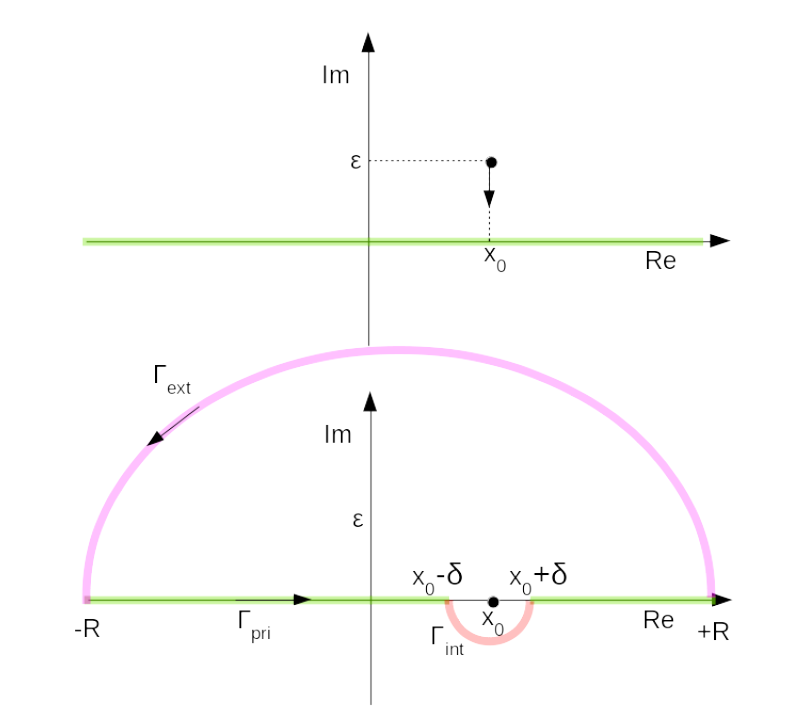
\includegraphics{image003.png}
    \caption{Integration path for an indented integral\label{fig:indented1}}
\end{figure}

 




\end{document}
